\section{Demonstration und Auswertung}


\subsection{Geschaffene Lösung}

Im Rahmen dieser Arbeit entstand eine Lösung zur Aggregation und Betrachtung der Daten des Argo-Programms. Unter dem Argo-Programm werden Messwerte über den Klimazustand unserer Weltmeere gemessen und öffentlich gemacht. Diese Daten wurden hier Heruntergeladen, angepasst und in ein Format überführt, dass durch eine Webapplikation zur Anzeige gebracht werden konnte. Die Webdarstellung bediente sich moderner Frameworks wie Flask, SQLAlchemy und OpenLayers um die Daten über eine Weltkarte zur Darstellung zu bringen. Durch die Kartenrepräsentation der Messstation ist es den Anwendern möglich mit den Datensätzen zu interagieren. Durch einen Mausklick werden die Messwerte über Funktionsplots angezeigt.  Fehlerharte Daten werden markiert, so das es den Anwendenden möglich ist, diese zu erkennen.

\begin{figure}[H]
 \centering
 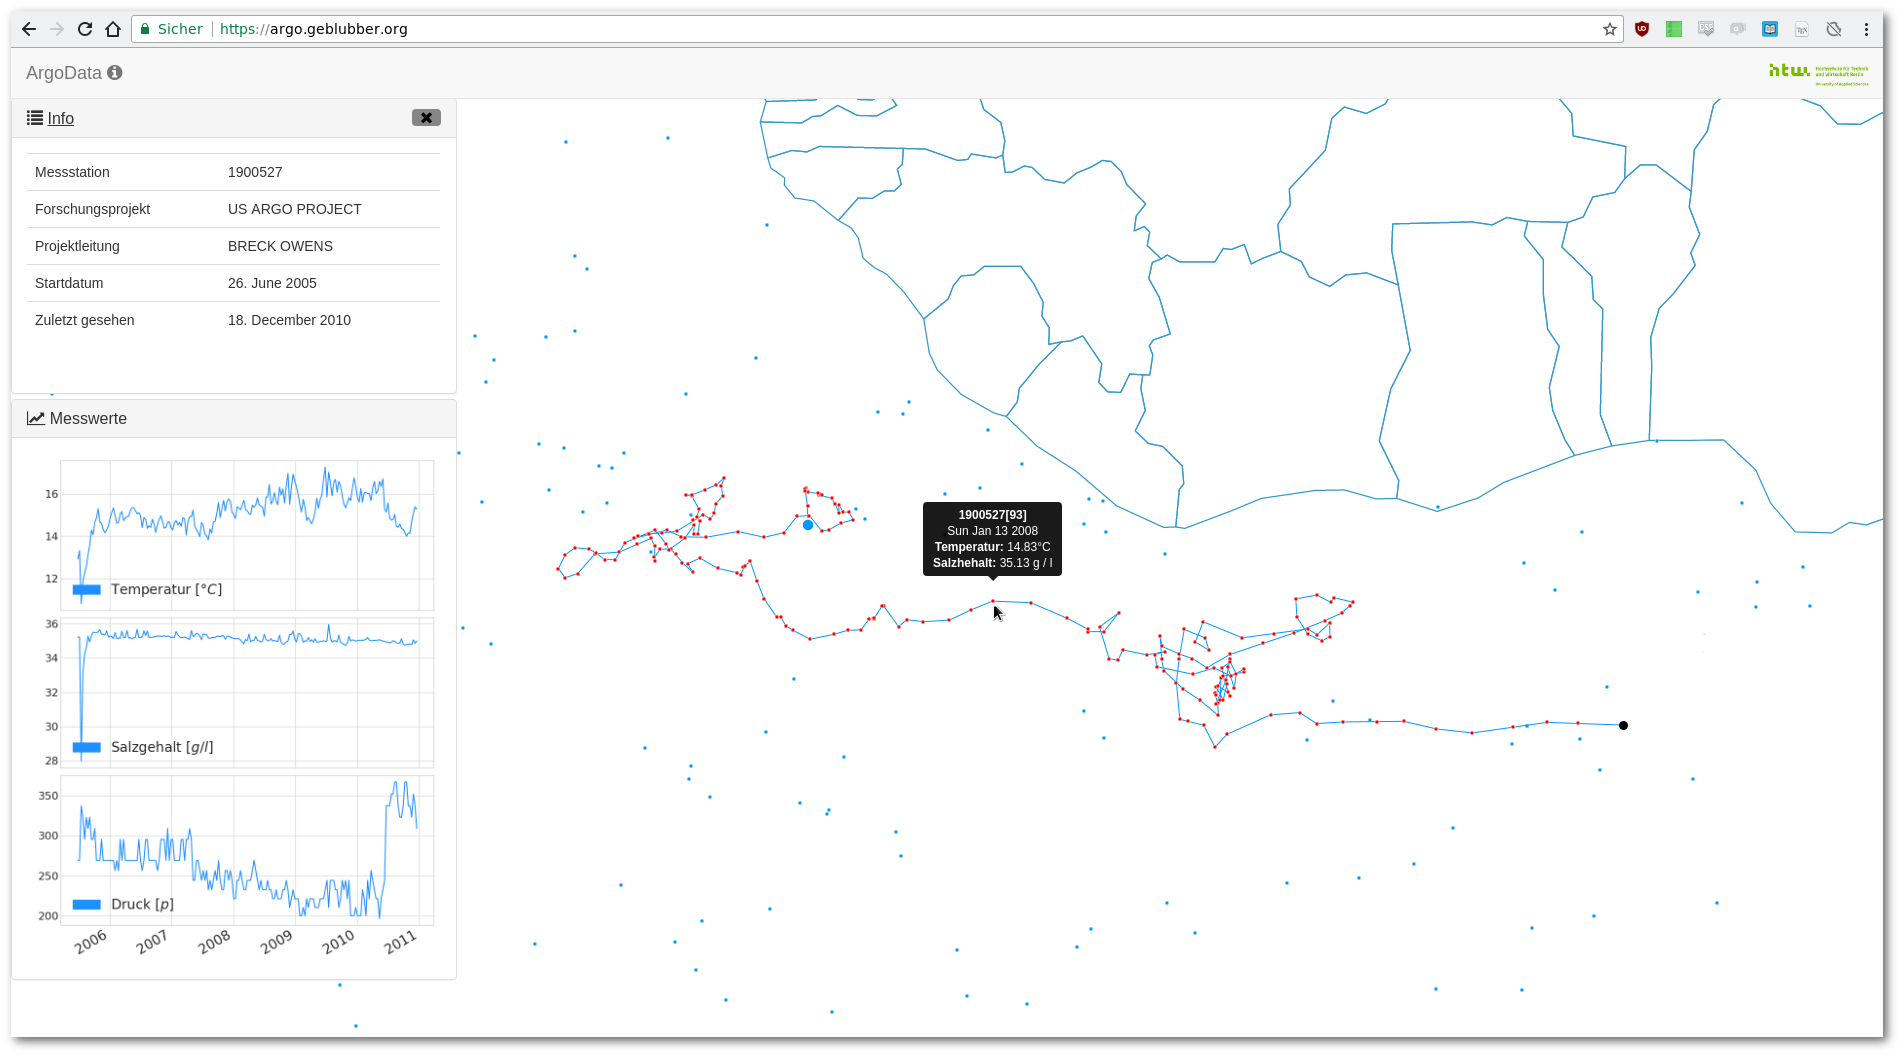
\includegraphics[width=\textwidth]{pix/argodata_complete.png}
 % argodata_complete.png: 1872x1026 px, 96dpi, 49.52x27.14 cm, bb=0 0 1404 769
 \caption{Die Webpräsenz von Argo-Data}
 \label{fig:argodataWeb}
\end{figure}

Bei der Aggregation wurde stark auf die Modularität der Anwendung geachtet. Objektorientierte Programmierung und die saubere Ausarbeitung von Schnittstellen wurde als zentrales Entwicklungsparadigma betrachtet. Auch in der Webanwendung wurde auf eine feinteilige Modularisierung geachtet. Die bei der Entwicklung mit Flask empfohlenen Entwurfsmuster wurden umgesetzt. 


\subsubsection{Erweiterungsmöglichkeiten}

Der hier ausgearbeite Prozess der Datenüberführung ist stark monolytisch und statisch ausgelegt. Es werden immer alle Daten erneuert, auch wenn dieser bereits in der Datenhaltung vorhanden sind. Dies ist als verbesserungswürdig anzusehen, da hier zum einen unnötige Schreibzugriffe stattfinden und zum anderen die Überführung der Daten in die produktive Datenhaltung Ausfallzeiten hervorrufen. Durch einen ständig laufenden Microservice, der die Daten nur auf Veränderungen hin untersucht und diese Nachträgt könnte die Anwendung somit stark verbessert werden. 


Durch die Usability Umfrage wurde ermittelt, dass sich die Benutzer verloren fühlten, bzw. eine Hilfestellung erwartet hätten. Hier könnte man durch ein Interface-Overlay oder der initialen Anzeige eines Hilfsmodals eine bessere Hilfestellung leisten.

Die Anforderung der Messdaten und das Erstellen des Funktionsplots erfordert nach jedem Klick einige Sekunden, bis die Daten zur Anzeige gebracht werden. Dadurch wirkt die Darstellung schwerfällig und träge. Diesem könnte man durch einen Caching-Prozess entgegenwirken. Ein weiterer spannender Ansatz wäre das proaktive Laden von Datensätzen durch Ermittlung der Mauszeigerposition noch bevor der Datensatz angeklickt wurde. Dies könnte durch Maschinelles Lernen sogar noch weiter Verfeinert werden. Besonders die Kombination von Caches und dem proaktiven Laden der Daten könnte hier starke Verbesserung in der Seitengeschwindigkeit bringen. 



\newpage


\vspace*{\fill}\thispagestyle{plain}
Der echte Zug des Wissens ist nichts Statisches, das man anhalten und in Teile zerlegen kann. Er ist immer in Fahrt. Auf einem Gleis namens Qualität. Und die Lok und die 120 Güterwagen fahren nie woanders hin, als wo das Gleis der Qualität sie hinführt.
\\
\hrulefill \vspace{0.3cm}
\textbf{Robert M. Pirsing} -- \textit{Zen und die Kunst ein Motorrad zu warten}
\vspace*{\fill}
